\documentclass[11pt,a4paper]{article}
\usepackage[utf8]{inputenc}
\usepackage[T1]{fontenc}
\IfFileExists{lmodern.sty}{\usepackage{lmodern}}{}
\IfFileExists{spanish.ldf}{\usepackage[spanish,es-noshorthands]{babel}}{}
\usepackage{amsmath,amssymb,amsthm,mathtools}
\usepackage{enumitem}
\usepackage[margin=2.5cm]{geometry}
\usepackage{tikz}
\usepackage{booktabs}
\usepackage[colorlinks=true,linkcolor=blue!50!black,urlcolor=blue!50!black]{hyperref}
\setlength{\parskip}{3pt}
\linespread{1.04}

\newcommand{\Spec}{\operatorname{Spec}}
\newcommand{\Proj}{\operatorname{Proj}}
\newcommand{\Bl}{\operatorname{Bl}}
\newcommand{\gr}{\operatorname{gr}}
\newcommand{\nil}{\operatorname{nil}}
\newcommand{\ZZ}{\mathbb{Z}}
\newcommand{\QQ}{\mathbb{Q}}
\newcommand{\RR}{\mathbb{R}}
\newcommand{\CC}{\mathbb{C}}
\newcommand{\FF}{\mathbb{F}}
\newcommand{\A}{\mathbb{A}}
\newcommand{\PP}{\mathbb{P}}
\newcommand{\pp}{\mathfrak{p}}
\newcommand{\qq}{\mathfrak{q}}
\newcommand{\mm}{\mathfrak{m}}
\newcommand{\aaa}{\mathfrak{a}}
\newcommand{\bbb}{\mathfrak{b}}
\newcommand{\gen}[1]{\langle #1\rangle}

\theoremstyle{plain}
\newtheorem{teorema}{Teorema}[section]
\newtheorem{proposicion}[teorema]{Proposición}
\newtheorem{lema}[teorema]{Lema}
\newtheorem{corolario}[teorema]{Corolario}
\theoremstyle{definition}
\newtheorem{definicion}[teorema]{Definición}
\newtheorem{ejemplo}[teorema]{Ejemplo}
\theoremstyle{remark}
\newtheorem*{obs}{Observación}
\newtheorem*{docente}{Para el docente}

\newcounter{ej}
\newenvironment{ejercicio}[1][]{\refstepcounter{ej}\par\medskip\noindent\textbf{Ejercicio \theej}\ifx&#1&\else\ (#1)\fi.\ }{\par}
\newcommand{\proy}[1]{\par\smallskip\noindent\fbox{\parbox{0.94\linewidth}{\textbf{En el proyecto.} #1}}\par\smallskip}
\newcommand{\pregunta}[1]{\par\smallskip\noindent\fbox{\parbox{0.94\linewidth}{\textbf{Pregunta para la clase.} #1}}\par\smallskip}

\title{\textbf{Clase: Ideales, ideales primos y maximales}\\[4pt]
\large Sesión de 2 horas --- prerrequisito algebraico del proyecto sobre blow-ups}
\author{}
\date{Octubre de 2026}

\begin{document}
\maketitle

\section*{Ficha de la clase}

\paragraph{Público.} Estudiantes de posgrado que han llevado álgebra de pregrado (anillos, homomorfismos, anillos cociente, dominios, DIP y DFU, anillos de polinomios). La clase fija el vocabulario de ideales que usa todo el proyecto: el centro de un blow-up es un ideal, el álgebra de Rees se construye con sus potencias, y los puntos de $\Spec A$ son sus ideales primos.

\paragraph{Objetivos.} Al terminar, el estudiante podrá:
\begin{enumerate}[itemsep=1pt]
\item decidir si un subconjunto es un ideal y si es propio;
\item calcular el ideal generado por un conjunto, sus sumas, productos y potencias;
\item decidir, con la caracterización por cocientes, si un ideal es primo, maximal o radical;
\item usar la correspondencia entre ideales de $A/I$ e ideales de $A$ que contienen a $I$;
\item reconocer los ideales que aparecen en el proyecto: ideal de un punto, ideal de una curva, centros de blow-up y el ideal $(x^2,y)$ de los blow-ups con pesos.
\end{enumerate}

\paragraph{Cronograma.}
\begin{center}
\begin{tabular}{@{}lll@{}}
\toprule
Bloque & Contenido & Tiempo \\
\midrule
0 & Motivación & 5 min \\
1 & Ideales e ideales propios & 20 min \\
2 & Ideal generado; suma, producto, potencias & 25 min \\
\multicolumn{3}{c}{\emph{pausa (5 min)}} \\
3 & Ideales primos y maximales; radical & 30 min \\
4 & Correspondencia y homomorfismos & 10 min \\
5 & Ideales del proyecto & 10 min \\
6 & Ejercicios & 15 min \\
\bottomrule
\end{tabular}
\end{center}

\paragraph{Convención.} Todos los anillos son conmutativos con unidad. $k$ es un cuerpo; si se dice algebraicamente cerrado, se indica.

\section{Bloque 0. Motivación (5 min)}

En grupos, la teoría se organiza con los \emph{subgrupos normales}: son los núcleos de los homomorfismos. En anillos, los núcleos son los \emph{ideales}. Son además lo que se necesita para ``quitar'' elementos al hacer un cociente: $\ZZ/12$, $k[x]/(x^2)$, $k[x,y]/(y^2-x^3)$.

Pero en geometría algebraica los ideales son mucho más: son \emph{geometría}. Un ideal $I\subset k[x,y]$ define el conjunto de puntos donde todos sus elementos se anulan; el ideal $(x,y)$ define el origen, $(y-x^2)$ una parábola, $(xy)$ la cruz de los dos ejes. Y en este proyecto, el blow-up de $\A^2$ \emph{a lo largo de un ideal} $I$ es el objeto central. Hoy aprendemos a manejar ideales.

\section{Bloque 1. Ideales e ideales propios (20 min)}

\begin{definicion}[Ideal]
Sea $A$ un anillo. Un subconjunto $I\subseteq A$ es un \emph{ideal} si
\begin{enumerate}[label=(\roman*),itemsep=1pt]
\item $0\in I$ y $a+b\in I$ para $a,b\in I$ (subgrupo aditivo);
\item $ra\in I$ para todo $r\in A$ y $a\in I$ (absorbe el producto por elementos de $A$).
\end{enumerate}
\end{definicion}

La condición (ii) es la diferencia con un subanillo: un ideal no tiene por qué contener a $1$, pero si lo contiene, es todo.

\begin{ejemplo}[Ideales y no ideales]\label{ej:ideales}
\begin{enumerate}[label=(\alph*),itemsep=2pt]
\item En $\ZZ$: $n\ZZ=(n)$ es un ideal. Todo ideal de $\ZZ$ es de esta forma.
\item En $k[x]$: $(x-a)=\{f:f(a)=0\}$ es un ideal (si $f(a)=0$ y $g$ es cualquier polinomio, $(gf)(a)=0$).
\item En $k[x,y]$: $\mm_0=\{f:f(0,0)=0\}$ es un ideal, formado por los polinomios sin término constante.
\item \emph{El núcleo de un homomorfismo} $\varphi:A\to B$ es un ideal: si $\varphi(a)=0$ entonces $\varphi(ra)=\varphi(r)\cdot0=0$.
\item \emph{No ideal:} $\ZZ\subset\QQ$ es un subanillo pero no un ideal: $\tfrac12\cdot1\notin\ZZ$.
\item \emph{No ideal:} $(2)\cup(3)=\{\text{múltiplos de 2 o de 3}\}\subset\ZZ$ no es un ideal: $2+3=5\notin(2)\cup(3)$. (La unión de ideales casi nunca es ideal.)
\item \emph{No ideal:} en $k[x]$, $\{f:f(0)=1\}$ no contiene a $0$.
\end{enumerate}
\end{ejemplo}

\paragraph{Todo ideal es un núcleo.} Para un ideal $I$, el homomorfismo canónico $\pi:A\to A/I$ tiene núcleo $I$. Así \emph{ideales $=$ núcleos de homomorfismos}, y el anillo cociente $A/I$ es el recipiente donde ``$I$ vale cero''.

\subsection{Ideales propios}

\begin{definicion}[Ideal propio]
Un ideal $I$ es \emph{propio} si $I\ne A$. Los ideales \emph{triviales} son $(0)$ y $A$.
\end{definicion}

\paragraph{Cuidado con el vocabulario.} Aquí ``propio'' significa $I\ne A$ (como en la definición de ideal primo y maximal). En algunos textos ``propio'' significa ``distinto de $0$ y de $A$''; el libro de Palacios y el resto de este proyecto usan la primera acepción.

\begin{lema}\label{lema:propio}
Para un ideal $I$ de $A$ son equivalentes: (a) $I=A$; (b) $1\in I$; (c) $I$ contiene una unidad. En consecuencia, un ideal es propio si y sólo si no contiene unidades.
\end{lema}
\begin{proof}
(a)$\Rightarrow$(b) es trivial. (b)$\Rightarrow$(c): $1$ es unidad. (c)$\Rightarrow$(a): si $u\in I$ es unidad, para todo $a\in A$ se tiene $a=(au^{-1})u\in I$.
\end{proof}

\begin{corolario}[Los cuerpos]\label{cor:cuerpo}
Un anillo $K\ne0$ es un cuerpo si y sólo si sus únicos ideales son $(0)$ y $K$.
\end{corolario}
\begin{proof}
Si $K$ es cuerpo y $I\ne0$, existe $a\in I$ no nulo, que es una unidad: $I=K$ por el Lema~\ref{lema:propio}. Recíprocamente, si los únicos ideales son $(0)$ y $K$, para $a\ne0$ el ideal $(a)$ es no nulo, luego $(a)=K\ni1$, es decir $1=ab$ para algún $b$.
\end{proof}

\pregunta{¿Cuántos ideales tiene $\ZZ/12$? ¿Y $k[x]/(x^2)$? ¿Y $\QQ$?}

\emph{Respuesta.} $\QQ$: dos (por el Corolario~\ref{cor:cuerpo}). $k[x]/(x^2)$: tres, $(0)$, $(\bar x)$ y todo. $\ZZ/12$: seis, correspondientes a los divisores de $12$ (se justifica con el Teorema~\ref{teo:corresp}).

\begin{docente}
Pedir a los estudiantes que justifiquen en voz alta por qué $(a,b)=A$ si $a,b$ son coprimos en $\ZZ$: ``porque existen $u,v$ con $ua+vb=1$ (Bézout), y entonces $1\in(a,b)$ por el Lema~\ref{lema:propio}''. Es la primera instancia de ``generado por'' que aparece enseguida.
\end{docente}

\section{Bloque 2. Ideal generado; suma, producto y potencias (25 min)}

\subsection{El ideal generado}

\begin{definicion}[Ideal generado]
Para $S\subseteq A$, el \emph{ideal generado por $S$}, $\gen S$, es la intersección de todos los ideales que contienen a $S$; es el \emph{menor} ideal que contiene a $S$. Un ideal es \emph{finitamente generado} si $I=\gen{f_1,\dots,f_r}$; es \emph{principal} si $I=(f)=\gen f$.
\end{definicion}

\begin{proposicion}\label{prop:generado}
$\gen S=\Big\{\sum_{i=1}^na_is_i:\ n\ge0,\ a_i\in A,\ s_i\in S\Big\}$ (combinaciones lineales finitas con coeficientes en $A$). En particular $\gen{f_1,\dots,f_r}=\{a_1f_1+\cdots+a_rf_r\}$ y $(f)=\{af:a\in A\}=fA$.
\end{proposicion}
\begin{proof}
El conjunto $J$ de combinaciones lineales es un ideal (cerrado por sumas y por multiplicación por elementos de $A$) y contiene a $S$. Todo ideal que contiene a $S$ contiene todas las combinaciones lineales, luego contiene a $J$. Así $J$ es el menor.
\end{proof}

\begin{ejemplo}[Generadores concretos]\label{ej:gen}
\begin{enumerate}[label=(\alph*),itemsep=2pt]
\item En $\ZZ$: $\gen{6,10}=(2)$, porque $\gcd(6,10)=2=2\cdot 6-1\cdot 10$ (Bézout) y todo elemento de $\gen{6,10}$ es múltiplo de $2$. $\gen{6,10,15}=\ZZ$ pues $\gcd=1$. En general $\gen{a,b}=(\gcd(a,b))$: \emph{en un DIP todo ideal finitamente generado es principal}.
\item En $k[x]$: $\gen{x^2-1,x^2-x}=(x-1)$, pues $\gcd(x^2-1,x^2-x)=x-1$.
\item En $k[x,y]$: $\gen{x,y}=\mm_0$, el ideal de todos los polinomios que se anulan en el origen: $f=f(0,0)+xg+yh$.
\item $\gen{x,y}$ \emph{no es principal}. Si fuera $(h)$, entonces $h\mid x$ y $h\mid y$. De $h\mid x$ se sigue que $h$ es constante no nula o $h=cx$; de $h\mid y$, que $h$ es constante no nula o $h=c'y$. Luego $h$ es una constante no nula, es decir una unidad, y $(h)=k[x,y]$. Pero $1\notin\gen{x,y}$ (todo elemento se anula en el origen). Contradicción. \emph{Moraleja:} $k[x,y]$ no es un DIP.
\item $\gen{x^2,xy,y^2}=\gen{x,y}^2$ (se verá en la Proposición~\ref{prop:potencias}).
\end{enumerate}
\end{ejemplo}

\begin{obs}
Un mismo ideal tiene muchos conjuntos de generadores: $\gen{x,y}=\gen{x,x+y}=\gen{x+y,x-y}$ (si $\operatorname{car}k\ne2$). Lo que no cambia es el ideal. En geometría, \emph{cambios de coordenadas lineales} (como $x\mapsto x+y$) no alteran el blow-up.
\end{obs}

\subsection{Operaciones con ideales}

\begin{definicion}
Sean $I,J$ ideales. Se definen: $I+J=\{a+b:a\in I,b\in J\}=\gen{I\cup J}$; $I\cap J$; $IJ=\gen{ab:a\in I,b\in J}$; $I^n=I\cdot I\cdots I$ ($n$ factores), $I^0=A$.
\end{definicion}

Siempre $IJ\subseteq I\cap J\subseteq I,J\subseteq I+J$.

\begin{ejemplo}\label{ej:operaciones}
\begin{enumerate}[label=(\alph*),itemsep=2pt]
\item En $\ZZ$: $(a)+(b)=(\gcd(a,b))$, $(a)\cap(b)=(\operatorname{lcm}(a,b))$, $(a)(b)=(ab)$. Con $a=4$, $b=6$: $(4)+(6)=(2)$, $(4)\cap(6)=(12)$, $(4)(6)=(24)\subsetneq(12)$: el producto puede ser estrictamente menor que la intersección.
\item En $k[x,y]$: $(x)(y)=(xy)=(x)\cap(y)$ (aquí coinciden). Pero $(x)(x)=(x^2)\subsetneq(x)=(x)\cap(x)$.
\item $(x)+(y)=\gen{x,y}$.
\item $(2)+(3)=\ZZ$: por el Lema~\ref{lema:propio}, $1=3-2\in(2)+(3)$.
\end{enumerate}
\end{ejemplo}

\subsection{Potencias de un ideal}

Las potencias $I^n$ son el ingrediente del \emph{álgebra de Rees} $R(I)=\bigoplus_{n\ge0}I^nt^n$ del proyecto: sin entenderlas, no hay blow-ups.

\begin{proposicion}[Generadores de las potencias]\label{prop:potencias}
Si $I=\gen{f_1,\dots,f_r}$, entonces $I^n$ está generado por los monomios $f_1^{\alpha_1}\cdots f_r^{\alpha_r}$ con $\alpha_1+\cdots+\alpha_r=n$. En particular, $I^n$ se genera con $\binom{n+r-1}{r-1}$ elementos.
\end{proposicion}
\begin{proof}
Todo elemento de $I^n$ es suma de productos $a_1\cdots a_n$ con $a_j\in I$. Cada $a_j=\sum_i r_{ji}f_i$; al desarrollar el producto queda una combinación $A$-lineal de monomios de grado $n$ en los $f_i$. Recíprocamente esos monomios están en $I^n$.
\end{proof}

\begin{ejemplo}\label{ej:pot}
\begin{enumerate}[label=(\alph*),itemsep=2pt]
\item $\gen{x,y}^n$ está generado por $x^n,x^{n-1}y,\dots,y^n$: $n+1$ generadores. Ejemplos: $\gen{x,y}^2=\gen{x^2,xy,y^2}$ y $\gen{x,y}^3=\gen{x^3,x^2y,xy^2,y^3}$. Una $f\in\gen{x,y}^n$ si y sólo si todos sus monomios tienen grado total $\ge n$.
\item $\gen{x^2,y}^2=\gen{x^4,x^2y,y^2}$: $3$ generadores. Nótese que $\gen{x^2,y}^2\ne\gen{x,y}^4$.
\item $(f)^n=(f^n)$ para un ideal principal.
\end{enumerate}
\end{ejemplo}

\proy{Para un ideal $I=\gen{f_0,\dots,f_r}$, el álgebra de Rees $R(I)=\bigoplus I^nt^n$ está generada sobre $A$ por $f_0t,\dots,f_rt$, y esto \emph{es} la Proposición~\ref{prop:potencias}: $I^nt^n$ está generado por los monomios de grado $n$ en los $f_it$. Eso da la inmersión del blow-up en $\PP^r_A$. Para $I=\gen{x,y}$ el cálculo de $I^n/I^{n+1}$ es el contenido de la Sección~\ref{sec:proy} y da la dimensión $n+1$ que aparece en la función de Hilbert.}

\begin{docente}
Pausa de 5 minutos. Dejar planteado: ``¿Cuántos ideales primos tiene $\ZZ$? ¿Y $k[x]$? ¿Cuáles son maximales?'' Es el puente al bloque siguiente.
\end{docente}

\section{Bloque 3. Ideales primos y maximales (30 min)}

\begin{definicion}
Sea $\pp\subset A$ un ideal propio. Es \emph{primo} si $ab\in\pp\Rightarrow a\in\pp$ o $b\in\pp$. Un ideal propio $\mm$ es \emph{maximal} si no existe un ideal propio $J$ con $\mm\subsetneq J$.
\end{definicion}

\paragraph{Intuición.} Primo $\approx$ ``no se factoriza'' (como el número primo $p$, que si divide a $ab$ divide a $a$ o a $b$). Maximal $\approx$ ``lo más grande posible sin ser todo''. En $\Spec$: primo = punto, maximal = punto cerrado.

\subsection{Caracterización por cocientes}

\begin{teorema}\label{teo:cocientes}
Sea $I\subsetneq A$ un ideal propio.
\begin{enumerate}[label=(\alph*),itemsep=1pt]
\item $I$ es primo $\iff A/I$ es un dominio.
\item $I$ es maximal $\iff A/I$ es un cuerpo.
\end{enumerate}
En consecuencia, \emph{todo ideal maximal es primo}.
\end{teorema}
\begin{proof}
(a) $ab\in I\iff\bar a\bar b=0$ en $A/I$; ``$ab\in I\Rightarrow a\in I$ o $b\in I$'' es exactamente ``$\bar a\bar b=0\Rightarrow\bar a=0$ o $\bar b=0$''; además $A/I\ne0$ porque $I$ es propio.

(b) Por el Teorema~\ref{teo:corresp} más abajo, los ideales de $A/I$ corresponden a los ideales de $A$ que contienen a $I$. Entonces $I$ es maximal $\iff$ $A/I$ sólo tiene los ideales $(0)$ y $A/I$ $\iff A/I$ es cuerpo (Corolario~\ref{cor:cuerpo}).

Finalmente, un cuerpo es un dominio.
\end{proof}

\paragraph{La recíproca es falsa.} $(0)\subset\ZZ$ es primo ($\ZZ$ es dominio) pero no maximal ($\ZZ$ no es cuerpo).

\begin{teorema}[Existencia de maximales]
Todo ideal propio está contenido en un ideal maximal.
\end{teorema}
\begin{proof}[Idea]
Se aplica el lema de Zorn al conjunto de ideales propios que contienen a $I$, ordenado por inclusión: la unión de una cadena de ideales propios es un ideal propio (no contiene a $1$). En un anillo noetheriano (el caso del proyecto) basta una cadena ascendente finita.
\end{proof}

\subsection{Ejemplos}

\begin{ejemplo}[{En $\ZZ$ y en $k[x]$}]\label{ej:primos1}
\begin{itemize}[itemsep=2pt]
\item En $\ZZ$: $(n)$ es primo $\iff n=0$ ó $n=\pm p$ con $p$ primo; $(n)$ es maximal $\iff n=\pm p$. El cociente $\ZZ/(p)=\FF_p$ es un cuerpo.
\item En un DIP (como $\ZZ$ o $k[x]$): todo primo no nulo es maximal. Si $(p)\subseteq(q)\ne A$, entonces $q\mid p$ y como $p$ es irreducible, $q$ es asociado de $p$ o unidad; así $(q)=(p)$.
\item En $k[x]$: $(f)$ es primo $\iff f$ irreducible $\iff(f)$ es maximal ($f\ne0$). Si $k$ es algebraicamente cerrado los irreducibles son $x-a$ y $k[x]/(x-a)\cong k$ vía $f\mapsto f(a)$.
\item \emph{Depende del cuerpo.} $(x^2+1)$ es maximal en $\RR[x]$ (cociente $\RR[x]/(x^2+1)\cong\CC$) y en $\QQ[x]$ (cociente $\QQ(i)$), pero \emph{no es primo} en $\CC[x]$: $x^2+1=(x-i)(x+i)$ con ningún factor en el ideal.
\end{itemize}
\end{ejemplo}

\begin{ejemplo}[{En $k[x,y]$}]\label{ej:primos2}
Sea $A=k[x,y]$. Calculamos el cociente en cada caso:
\begin{itemize}[itemsep=2pt]
\item $(x)$: $A/(x)\cong k[y]$ (evaluar $x=0$). Dominio, no cuerpo: \emph{primo no maximal}. Geométricamente, el eje $y$.
\item $\gen{x,y}$: $A/\gen{x,y}\cong k$ (evaluar en el origen). Cuerpo: \emph{maximal}. Es el ideal del origen.
\item $\gen{x-a,y-b}$: $A/\gen{x-a,y-b}\cong k$ por evaluación en $(a,b)$; maximal. Si $k$ es algebraicamente cerrado, estos son \emph{todos} los maximales (Nullstellensatz).
\item $(y-x^2)$: la aplicación $A\to k[t]$, $x\mapsto t$, $y\mapsto t^2$ es sobreyectiva con núcleo $(y-x^2)$ (se sustituye $y=x^2$), luego $A/(y-x^2)\cong k[t]$: \emph{primo no maximal}. La parábola.
\item $(xy)$: \emph{no primo}, pues $x\cdot y\in(xy)$ y ni $x$ ni $y$ lo están. Corresponde a la unión de los dos ejes.
\item $\gen{x^2,y}$: \emph{no primo} (ver abajo) ni maximal (está contenido en $\gen{x,y}$). El cociente $A/\gen{x^2,y}\cong k[x]/(x^2)$ tiene nilpotentes: \emph{no es un dominio}.
\end{itemize}
\end{ejemplo}

\begin{ejemplo}[$y^2-x^3$ es primo]\label{ej:cuspide}
Sea $\varphi:k[x,y]\to k[t]$, $x\mapsto t^2$, $y\mapsto t^3$. Su imagen es $k[t^2,t^3]$. \emph{Afirmación:} $\ker\varphi=(y^2-x^3)$. Es claro que $y^2-x^3\in\ker\varphi$. Recíprocamente, dividiendo por el polinomio mónico $y^2-x^3\in k[x][y]$, todo $g$ se escribe $g=q\,(y^2-x^3)+a(x)+b(x)y$. Si $\varphi(g)=0$: $a(t^2)+b(t^2)t^3=0$; el primer sumando sólo tiene potencias pares de $t$ y el segundo sólo impares, así $a=b=0$ y $g\in(y^2-x^3)$. Entonces
\[
k[x,y]/(y^2-x^3)\cong k[t^2,t^3]\subset k[t],
\]
que es un dominio (subanillo de $k[t]$). Por el Teorema~\ref{teo:cocientes}, $(y^2-x^3)$ es primo. \emph{No es maximal}: $k[t^2,t^3]$ no es un cuerpo.
\end{ejemplo}

\pregunta{¿Es $\gen{x^2,y}$ primo? ¿Por qué? (Pista: ¿existen $a,b\notin I$ con $ab\in I$?)}

\emph{Respuesta.} No: $x\cdot x=x^2\in I$ pero $x\notin I$. Tampoco es radical: $x\in\sqrt I\setminus I$.

\subsection{Primos y productos de ideales}

\begin{proposicion}\label{prop:primoprod}
Sea $\pp$ primo e $I,J$ ideales con $IJ\subseteq\pp$. Entonces $I\subseteq\pp$ o $J\subseteq\pp$. En particular $I\cap J\subseteq\pp\Rightarrow I\subseteq\pp$ o $J\subseteq\pp$.
\end{proposicion}
\begin{proof}
Si $I\not\subseteq\pp$, hay $a\in I\setminus\pp$. Para cada $b\in J$, $ab\in IJ\subseteq\pp$ y $a\notin\pp$, luego $b\in\pp$. Así $J\subseteq\pp$. Para la segunda afirmación, $IJ\subseteq I\cap J$.
\end{proof}

Este resultado es la razón de que ``irreducible'' en $\Spec$ corresponda a ``primo'' en álgebra: si $V(\aaa)=V(\bbb_1)\cup V(\bbb_2)$, entonces $\bbb_1\bbb_2\subseteq\sqrt\aaa$.

\subsection{El radical}

\begin{definicion}
El \emph{radical} de un ideal $I$ es $\sqrt I=\{a\in A:a^n\in I\text{ para algún }n\ge1\}$. $I$ es \emph{radical} si $I=\sqrt I$. El \emph{nilradical} de $A$ es $\nil(A)=\sqrt{(0)}$.
\end{definicion}

\begin{proposicion}
$\sqrt I$ es un ideal que contiene a $I$. Todo ideal primo es radical.
\end{proposicion}
\begin{proof}
Si $a^m,b^n\in I$, entonces $(a+b)^{m+n-1}=\sum\binom{m+n-1}{i}a^ib^{m+n-1-i}$ y en cada término $i\ge m$ o $m+n-1-i\ge n$, luego todo término está en $I$. Para $r\in A$, $(ra)^m=r^ma^m\in I$. Si $\pp$ es primo y $a^n\in\pp$, entonces $a\in\pp$ (inducción sobre $n$).
\end{proof}

\begin{ejemplo}[Radicales]\label{ej:radicales}
\begin{center}
\begin{tabular}{@{}llll@{}}
\toprule
Ideal & Anillo & $\sqrt I$ & ¿Radical? \\
\midrule
$(12)$ & $\ZZ$ & $(6)$ & no \\
$(30)$ & $\ZZ$ & $(30)$ & sí (libre de cuadrados) \\
$(x^2)$ & $k[x]$ & $(x)$ & no \\
$\gen{x^2,y}$ & $k[x,y]$ & $\gen{x,y}$ & no \\
$\gen{x,y}^n$ & $k[x,y]$ & $\gen{x,y}$ & no si $n\ge2$ \\
$(xy)$ & $k[x,y]$ & $(xy)$ & sí (no primo) \\
$(y^2-x^3)$ & $k[x,y]$ & $(y^2-x^3)$ & sí (es primo) \\
\bottomrule
\end{tabular}
\end{center}
Regla: en $\ZZ$, $\sqrt{(n)}=(\text{producto de los primos que dividen a }n)$.
\end{ejemplo}

\paragraph{Resumen de las tres propiedades.}
\begin{center}
\begin{tabular}{@{}lccc@{}}
\toprule
Ideal $I$ en $k[x,y]$ & primo & maximal & radical \\
\midrule
$\gen{x,y}$ & sí & sí & sí \\
$(x)$, $(y-x^2)$, $(y^2-x^3)$ & sí & no & sí \\
$(xy)$ & no & no & sí \\
$\gen{x^2,y}$ & no & no & no \\
$\gen{x,y}^2$ & no & no & no \\
\bottomrule
\end{tabular}
\end{center}

\begin{center}
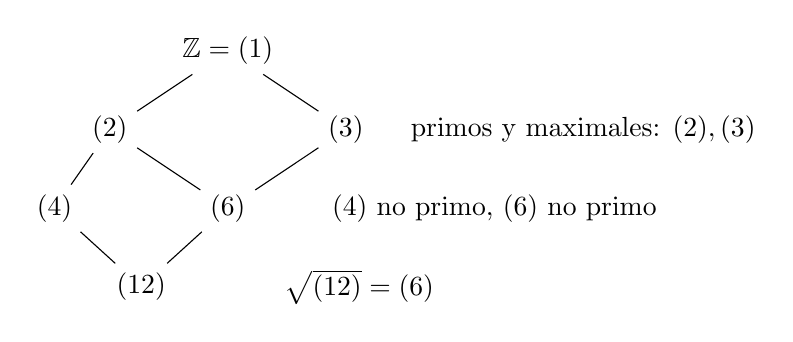
\begin{tikzpicture}[scale=1.0]
 \node (A) at (0,3) {$\ZZ=(1)$};
 \node (2) at (-1.5,2) {$(2)$}; \node (3) at (1.5,2) {$(3)$};
 \node (4) at (-2.2,1) {$(4)$}; \node (6) at (0,1) {$(6)$};
 \node (12) at (-1.1,0) {$(12)$};
 \draw (A)--(2); \draw (A)--(3); \draw (2)--(4); \draw (2)--(6); \draw (3)--(6); \draw (4)--(12); \draw (6)--(12);
 \node[right] at (2.2,2) {primos y maximales: $(2),(3)$};
 \node[right] at (1.2,1) {$(4)$ no primo, $(6)$ no primo};
 \node[right] at (0.6,0) {$\sqrt{(12)}=(6)$};
\end{tikzpicture}
\end{center}
\emph{Retículo de los ideales de $\ZZ$ que contienen a $(12)$.} Según la correspondencia (Teorema~\ref{teo:corresp}) son los ideales de $\ZZ/12$; los primos del cociente son $(2)/(12)$ y $(3)/(12)$.

\section{Bloque 4. Correspondencia y homomorfismos (10 min)}

\begin{teorema}[Correspondencia]\label{teo:corresp}
Sea $\pi:A\to A/I$ la proyección. Las aplicaciones $J\mapsto\pi(J)=J/I$ y $K\mapsto\pi^{-1}(K)$ son biyecciones inversas entre ideales de $A$ que contienen a $I$ e ideales de $A/I$. Conservan inclusiones, sumas e intersecciones. Además $J$ es primo (resp.~maximal) $\iff J/I$ es primo (resp.~maximal), pues $(A/I)/(J/I)\cong A/J$.
\end{teorema}
\begin{proof}[Idea]
$\pi$ es sobreyectivo, luego $\pi(\pi^{-1}(K))=K$; y si $J\supseteq I$, $\pi^{-1}(\pi(J))=J+I=J$. El isomorfismo $(A/I)/(J/I)\cong A/J$ es el tercer teorema de isomorfismo; con el Teorema~\ref{teo:cocientes} se concluye.
\end{proof}

\begin{ejemplo}
Los ideales primos de $k[x,y]/(xy)$ se corresponden con los primos de $k[x,y]$ que contienen a $(xy)$. Un primo que contiene a $xy$ contiene a $x$ o a $y$ (Proposición~\ref{prop:primoprod}). Los primos minimales son $(x)$ y $(y)$; los maximales con $k$ algebraicamente cerrado son $\gen{x,y-b}$, $\gen{x-a,y}$ (puntos de los ejes). \emph{Dos componentes irreducibles} en la cruz.
\end{ejemplo}

\begin{proposicion}[Contracción]\label{prop:contr}
Sea $\varphi:A\to B$ un homomorfismo y $\qq\subset B$ primo. Entonces $\varphi^{-1}(\qq)$ es primo. El análogo para maximales es falso: $\ZZ\hookrightarrow\QQ$, $(0)$ maximal en $\QQ$ y $\varphi^{-1}(0)=(0)$ no maximal en $\ZZ$.
\end{proposicion}
\begin{proof}
$1\notin\varphi^{-1}(\qq)$; si $ab\in\varphi^{-1}(\qq)$, entonces $\varphi(a)\varphi(b)\in\qq$ y uno de los dos está en $\qq$.
\end{proof}

\proy{La Proposición~\ref{prop:contr} es la que hace que un homomorfismo $A\to B$ induzca $\Spec B\to\Spec A$: en el proyecto, el morfismo estructural $\pi:\Bl_I X\to X$ viene de $A\to R(I)_{(ft)}=A[I/f]$, y $\varphi^*(\qq)=\varphi^{-1}(\qq)$ es la contracción.}

\section{Bloque 5. Los ideales del proyecto (10 min)}\label{sec:proy}

\begin{ejemplo}[Un punto: ideal maximal]
En $A=k[x,y]$, el ideal de un punto $p=(a,b)$ es $\mm_p=\{f:f(p)=0\}=\gen{x-a,y-b}$ y es maximal (núcleo de la evaluación $A\to k$, sobreyectiva). El blow-up de $\A^2$ en $p$ es $\Bl_{\mm_p}\A^2$.
\end{ejemplo}

\begin{ejemplo}[Una curva: ideal principal]
La curva $C=V(f)$ tiene ideal $(f)$. Por el Ejemplo~\ref{ej:cuspide}, $(y^2-x^3)$ es primo (la cúspide es irreducible); $(xy)$ no lo es (dos componentes). En $k[x,y]$ (DFU), $(f)$ es primo $\iff f$ irreducible.
\end{ejemplo}

\begin{ejemplo}[Multiplicidad y potencias de $\mm$]
Sea $\mm=\gen{x,y}$. Entonces $f\in\mm^n\iff$ todos los monomios de $f$ tienen grado $\ge n$ (Ejemplo~\ref{ej:pot}(a)). La \emph{multiplicidad} de $C=V(f)$ en el origen es $m=\max\{n:f\in\mm^n\}$. Así $y-x^2$ tiene $m=1$ (liso), $y^2-x^3$ y $xy$ tienen $m=2$ (singulares).
\end{ejemplo}

\begin{ejemplo}[Los cocientes $I^n/I^{n+1}$ y el divisor excepcional]\label{ej:gr}
Sea $A=k[x,y]$, $I=\mm=\gen{x,y}$. Como $\mm^n$ está generado por los monomios de grado $\ge n$, el cociente $\mm^n/\mm^{n+1}$ tiene base los $n+1$ monomios $x^iy^{n-i}$ de grado exactamente $n$. Entonces
\[
\gr_{\mm}(A)=\bigoplus_{n\ge0}\mm^n/\mm^{n+1}\cong k[x,y],
\]
con grados usuales, y el divisor excepcional del blow-up del origen es $\Proj\gr_\mm(A)=\Proj k[x,y]=\PP^1$. Para la cúspide, $B=k[x,y]/(y^2-x^3)$ con $\mm=\gen{x,y}B$: se obtiene $\gr_\mm(B)\cong k[x,y]/(y^2)$ (la forma inicial de $y^2-x^3$ es $y^2$) y $\dim\mm^n/\mm^{n+1}=1,2,2,2,\dots$: el divisor excepcional de la cúspide es un punto doble de $\PP^1$, $m=2$.
\end{ejemplo}

\begin{ejemplo}[Un centro que no es radical]
$I=\gen{x^2,y}$ no es primo ni radical ($\sqrt I=\gen{x,y}$), pero define un blow-up perfectamente válido: el blow-up con pesos $(1,2)$ de $\A^2$. Su carta $k[x,y,u]/(x^2-yu)$ tiene una singularidad (un punto doble $A_1$).
\end{ejemplo}

\begin{ejemplo}[Ideal principal: el blow-up no hace nada]
Si $I=(f)$ con $f$ no divisor de cero, $R(I)=\bigoplus f^nAt^n\cong A[T]$ con $T=ft$ y $\Proj A[T]=\Spec A$: $\Bl_{(f)}X=X$. Sólo los centros de codimensión $\ge2$ cambian la variedad.
\end{ejemplo}

\section{Bloque 6. Ejercicios (15 min en clase; el resto como tarea)}

\subsection*{Nivel A (en clase)}

\begin{ejercicio}
Complete la tabla: ¿es propio, primo, maximal, radical?
\begin{center}
\begin{tabular}{@{}ll@{}}
\toprule
Anillo & Ideales \\
\midrule
$\ZZ$ & $(12)$, $(7)$, $(0)$, $(1)$ \\
$\RR[x]$ & $(x^2-1)$, $(x^2+1)$ \\
$k[x,y]$ & $(x)$, $\gen{x,y}$, $(xy)$, $\gen{x^2,y}$, $(y-x^2)$ \\
\bottomrule
\end{tabular}
\end{center}
\end{ejercicio}

\begin{ejercicio}
Calcule $\gen{6,10,15}$ y $\gen{12,18}$ en $\ZZ$; y $\gen{x^2-1,x^3-1}$ en $\QQ[x]$.
\end{ejercicio}

\begin{ejercicio}
Escriba generadores de $\gen{x,y}^3$ y de $\gen{x^2,y}^2$. ¿Cuántos tiene cada uno?
\end{ejercicio}

\begin{ejercicio}
Pruebe que $\gen{x^2,y}$ no es principal en $k[x,y]$.
\end{ejercicio}

\subsection*{Nivel B (tarea)}

\begin{ejercicio}
Pruebe que $\sqrt I$ es un ideal y que $\sqrt{\gen{x^2,y}}=\gen{x,y}$.
\end{ejercicio}

\begin{ejercicio}
Halle todos los ideales de $\ZZ/12$. Indique cuáles son primos, cuáles maximales y el nilradical.
\end{ejercicio}

\begin{ejercicio}
Pruebe que $\gen{2,x}$ es un ideal maximal de $\ZZ[x]$ con cociente $\FF_2$, y que $(x)$ y $(2)$ son primos no maximales.
\end{ejercicio}

\begin{ejercicio}
Sea $\varphi:k[x,y]\to k[t]$, $x\mapsto t^2$, $y\mapsto t^3$. Verifique que $\ker\varphi=(y^2-x^3)$, y use $\varphi^{-1}(\gen{t})$ para identificar un ideal maximal de $k[x,y]$ que contiene a $(y^2-x^3)$.
\end{ejercicio}

\subsection*{Desafíos (Nivel C)}

\begin{ejercicio}
Pruebe que $\dim_k k[x,y]/\gen{x,y}^n=n(n+1)/2$. Calcule $\dim_k B/\mm^n$ para $B=k[x,y]/(y^2-x^3)$ y compárelo con la fórmula $nm-m(m-1)/2$ para $m=2$.
\end{ejercicio}

\begin{ejercicio}
Sea $\pp$ un primo de un anillo $A$ y $S=A\setminus\pp$. Pruebe que $\pp A_\pp$ es el único ideal maximal de $A_\pp=S^{-1}A$. (\emph{Anillo local}.)
\end{ejercicio}

\begin{ejercicio}
Sea $I=\gen{x,y}\subset k[x,y]$. Pruebe que $R(I)=\bigoplus I^nt^n\cong k[x,y,u,v]/(xv-yu)$ y que $I\cdot R(I)$ tiene cociente $\gr_I(A)\cong k[u,v]$. Deduzca que el divisor excepcional es $\PP^1$.
\end{ejercicio}

\section*{Soluciones y pistas}

\paragraph{Ejercicio 1.}
\begin{center}
\small
\begin{tabular}{@{}lllll@{}}
\toprule
Ideal & Propio & Primo & Maximal & Radical \\
\midrule
$(12)\subset\ZZ$ & sí & no & no & no ($\sqrt{}=(6)$) \\
$(7)$ & sí & sí & sí & sí \\
$(0)$ & sí & sí & no & sí \\
$(1)=\ZZ$ & no & no & no & sí \\
$(x^2-1)\subset\RR[x]$ & sí & no & no & sí \\
$(x^2+1)\subset\RR[x]$ & sí & sí & sí & sí \\
$(x)\subset k[x,y]$ & sí & sí & no & sí \\
$\gen{x,y}$ & sí & sí & sí & sí \\
$(xy)$ & sí & no & no & sí \\
$\gen{x^2,y}$ & sí & no & no & no \\
$(y-x^2)$ & sí & sí & no & sí \\
\bottomrule
\end{tabular}
\end{center}

\paragraph{Ejercicio 2.} $\gcd(6,10,15)=1$: $\gen{6,10,15}=\ZZ$. $\gen{12,18}=(6)$. $\gcd(x^2-1,x^3-1)=x-1$ (ambos se anulan en $1$; $x^2-1=(x-1)(x+1)$ y $x^3-1=(x-1)(x^2+x+1)$ con $x+1$ y $x^2+x+1$ coprimos): $\gen{x^2-1,x^3-1}=(x-1)$.

\paragraph{Ejercicio 3.} $\gen{x,y}^3=\gen{x^3,x^2y,xy^2,y^3}$ (4 generadores). $\gen{x^2,y}^2=\gen{x^4,x^2y,y^2}$ (3 generadores), por la Proposición~\ref{prop:potencias}.

\paragraph{Ejercicio 4.} Si $\gen{x^2,y}=(h)$, $h\mid y$ y $h\mid x^2$. De $h\mid y$: $h$ es constante no nula o $h=cy$. Si $h=cy$, $y\mid x^2$ es falso. Luego $h$ es constante no nula y $(h)=k[x,y]\ne\gen{x^2,y}$ (todo elemento de $\gen{x^2,y}$ se anula en el origen).

\paragraph{Ejercicio 5.} $\sqrt I$: si $a^m\in I$, $b^n\in I$, $(a+b)^{m+n-1}\in I$ (Proposición del radical); $(ra)^m\in I$. Para $I=\gen{x^2,y}$: $x\in\sqrt I$ ($x^2\in I$), $y\in I$, luego $\gen{x,y}\subseteq\sqrt I$; la otra inclusión: $\gen{x,y}$ es primo (luego radical) y contiene a $I$, así que $\sqrt I\subseteq\sqrt{\gen{x,y}}=\gen{x,y}$.

\paragraph{Ejercicio 6.} Los ideales de $\ZZ/12$ corresponden a divisores de $12$: $(\bar1),(\bar2),(\bar3),(\bar4),(\bar6),(\bar0)$, es decir seis. Primos (correspondiendo a $(2),(3)$): $(\bar2)$ y $(\bar3)$, ambos maximales (cocientes $\FF_2$, $\FF_3$). Nilradical: $(\bar6)=\sqrt{(\bar0)}$.

\paragraph{Ejercicio 7.} $\ZZ[x]/\gen{2,x}\cong\ZZ/2=\FF_2$ (evaluar $x=0$ y reducir módulo $2$): cuerpo, maximal. $\ZZ[x]/(x)\cong\ZZ$ es un dominio no cuerpo: $(x)$ primo no maximal. $\ZZ[x]/(2)\cong\FF_2[x]$: dominio no cuerpo: $(2)$ primo no maximal.

\paragraph{Ejercicio 8.} El núcleo es $(y^2-x^3)$ (Ejemplo~\ref{ej:cuspide}). $\varphi^{-1}(\gen t)=\{g:g(t^2,t^3)\in(t)\}=\{g:g(0,0)=0\}=\gen{x,y}$, maximal por el Ejemplo~\ref{ej:primos2}, y contiene a $y^2-x^3$ por ser $\ker\varphi\subseteq\varphi^{-1}(\gen t)$.

\paragraph{Ejercicio 9.} $\gen{x,y}^n$ tiene como base de $k[x,y]/\gen{x,y}^n$ los monomios de grado $<n$: hay $1+2+\cdots+n=n(n+1)/2$. Para $B$: $\dim\mm^j/\mm^{j+1}=1,2,2,2,\dots$, luego $\dim B/\mm^n=1+2(n-1)=2n-1$. La fórmula: $nm-m(m-1)/2=2n-1$ para $m=2$. Coinciden (para $n\ge1$).

\paragraph{Ejercicio 10.} Sea $\mm=\pp A_\pp$, formado por las fracciones $a/s$ con $a\in\pp$. Un elemento $a/s\notin\mm$ tiene $a\notin\pp$, luego $a\in S$ y $a/s$ es unidad con inverso $s/a$. Entonces el complemento de $\mm$ consiste en unidades. Todo ideal propio no contiene unidades, luego está dentro de $\mm$, que además es propio ($1\notin\mm$).

\paragraph{Ejercicio 11.} $\varphi:k[x,y,u,v]\to R(I)$, $u\mapsto xt$, $v\mapsto yt$, es sobreyectivo, graduado, y $xv-yu\mapsto xyt-yxt=0$. El cociente $k[x,y,u,v]/(xv-yu)$ es un dominio de dimensión $3$ (la cuádrica irreducible), igual que $R(I)$, luego el núcleo es exactamente $(xv-yu)$. Además $R(I)/IR(I)=\bigoplus I^n/I^{n+1}=\gr_I(A)$ (Ejemplo~\ref{ej:gr}), isomorfo a $k[u,v]$; entonces el divisor excepcional es $\Proj k[u,v]=\PP^1$.

\section*{Notas finales para el docente}

\begin{itemize}[itemsep=2pt]
\item \textbf{Errores frecuentes.} (i) Creer que la unión de ideales es un ideal. (ii) Usar ``propio'' como ``no nulo''. (iii) Pensar que primo $\Rightarrow$ maximal (el contraejemplo $(0)\subset\ZZ$ debe quedar grabado). (iv) Confundir $\gen{x,y}$ con $(x)\cup(y)$: es $(x)+(y)$. (v) Olvidar que $(x)^2=(x^2)\ne(x)$.
\item \textbf{Enlace con la clase siguiente.} Con este vocabulario, $\Spec A$ (clase sobre el Capítulo 5 de Palacios) es el conjunto de ideales primos con la topología $V(\aaa)$; los ejemplos de esta sesión son los puntos de esa geometría.
\item \textbf{Verificación sugerida.} Los ejemplos con $k[x,y]$ pueden comprobarse en Singular, Macaulay2 o con un CAS (sympy: \texttt{groebner}) para ver bases de Gröbner de $\gen{x^2,y}^2$ y la prueba de que $\ker\varphi=(y^2-x^3)$.
\end{itemize}

\end{document}
